\documentclass[10pt]{article}

% Set paper size and margins
\usepackage[a4paper, width=150mm, top=40mm, bottom=50mm, headsep=10mm, footskip=25mm]{geometry}

% Set line spacing
\renewcommand{\baselinestretch}{1.5}


\usepackage{graphicx}
\usepackage[table]{xcolor}
\usepackage{longtable}

\bibliographystyle{unsrt2authabbrvpp}
\begin{document}

% Title page
\begin{titlepage}
%	From model start & Remote learning & 0.1 \\
\centering
\vspace*{3cm}        
\huge
\textbf{Understanding how Victoria gained control of its second COVID-19 wave, Supplementary Appendix}
\vspace{0.5cm}
\end{titlepage}

% Table of contents
\clearpage
{
    \sffamily
    \tableofcontents
}
\clearpage

% This file describes the general structure of some of our tb_dynamics models.

\section{Model Structure}

\subsection{General features}

We use a deterministic compartmental model including six types of compartments that represent 
different states of infection and disease. The model uses the same conceptual approach and similar 
assumptions to previously published models \cite{trauer-2017, ragonnet-2019, ragonnet-2021, ragonnet-2022}. 
Here we describe the model structure without treatment compartment and related factors. 
\newline
A susceptible compartment (S) is used to represent individuals who have 
never been infected with \emph{Mycobacterium tuberculosis (M.tb)}. Latent TB infection (LTBI) is modelled 
using two successive compartments: early latent (E) and late latent (L) to capture the declining risk of 
disease progression over time from infection \cite{ragonnet-2017}. The active disease compartment (I) represents 
individuals who have progressed to the active stage of TB disease. Diseased individuals who recover 
through self-cure progress directly to the recovered compartment (R).
\newline
Non-TB-related mortality is modelled by applying death rates to all model compartments. In addition, 
disease-specific mortality is implemented by applying increased mortality rates to the active disease 
compartments (I).
\newline
Reinfection occurs in the model in two different ways. First, latently infected individuals may be 
reinfected, with this process modelled using a flow from the late latent (L) to the early latent 
compartment (E). Second, individuals who have recovered from TB disease may be reinfected and 
return to the early latent compartment. The structure of our model allows for differential risk of 
infection for the currently and previously infected individuals, compared to the infection-naive 
individuals.
\begin{figure}[!htp]
    \vspace*{-1cm}
    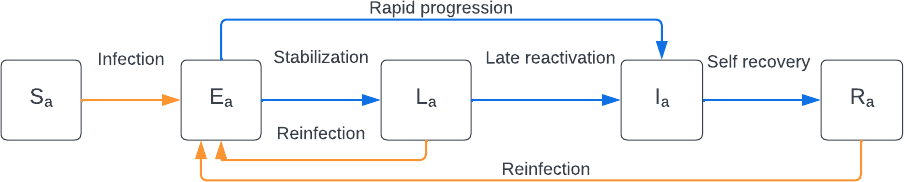
\includegraphics[width=\textwidth,height=\textheight,keepaspectratio]{images/model.png}
    \caption{Illustration of the model structure. 
    Boxes represent the different compartments types: susceptible (S), early latent (E), late latent (L), infectious (I), and recovered (R).
    The subscript indicates that compartments are stratified by age (a).}
    \label{fig:model}
\end{figure}

\subsection{Stratification by age}
The model is stratified using five categories: 0-4, 5-14, 15-34, 35-49 and 50+ years old. We assume 
heterogeneous mixing by age using an age-specific contact rate matrix. Since no local estimates of 
contact patterns by age were available for the Marshall Islands, we used a contact survey conducted in 
the Fijian population and adjusted the estimates to account for age distribution differences between
the two countries.


\subsection{Model stratification}
% Note that this will vary for every application, so will need to be edited - not sure of how best to manage this:
All compartments of the base compartmental structure were stratified by age, location and organ status:\linebreak
Age
\begin{itemize}
    \item Zero to 14 years
    \item 15 to 24 years
    \item 25 to 49 years
    \item 50 to 69 years
    \item 70 years and above
\end{itemize}
Location
\begin{itemize}
    \item South Tarawa
    \item Other location
\end{itemize}
Organ status
\begin{itemize}
    \item Pulmonary smear-posivtive
    \item Pulmonary smear-negative
    \item Extrapulmonary
\end{itemize}

\section{Clinical stratification} \label{clin}
% Note that this file describes only one implementation of the clinical stratification possible in the sm_sir code
The ``clinical" stratification acts by replicating each of the two age-stratified sequential compartments representing infectious COVID-19 into three categories.
The three clinical categories are:
\begin{enumerate}
    \item Asymptomatic persons
    \item Symptomatic persons who are never notified as cases
    \item Symptomatic persons who are successfully detected and notified
\end{enumerate}
For each age category, a proportion of new active infections are assumed to remain asymptomatic throughout their infectious period (specified in Table \ref{tab:age_params}).
This proportion remains fixed over time throughout a model run.
It is assumed that asymptomatic persons are never detected and so do not contribute to notifications.
The remaining proportion constitutes the second and third categories, comprising all persons developing symptomatic COVID-19 during their infectious period.
The proportion of these symptomatic persons who progress to the third category varies with time and is described under the section on case detection (Section \ref{cdr}).
\begin{figure}[ht]
    \begin{center}
    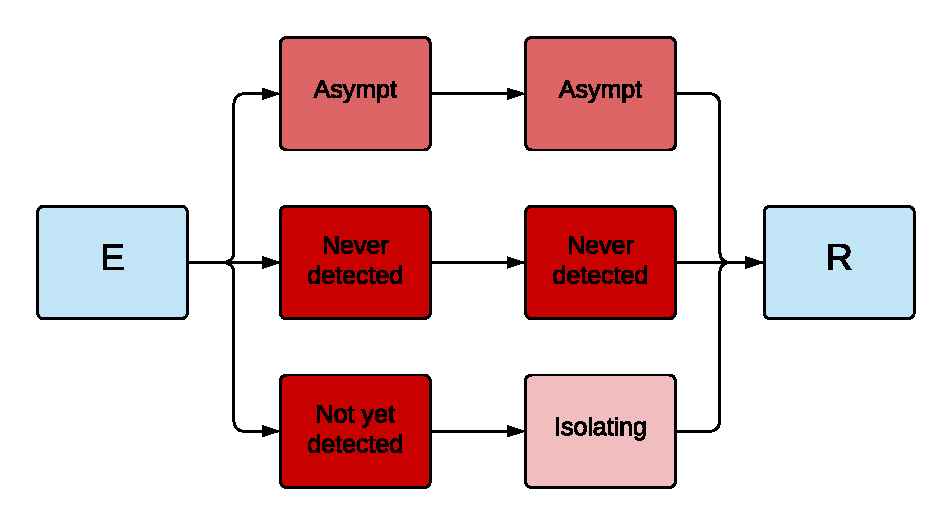
\includegraphics[width=0.7\textwidth]{../../tex_descriptions/models/sm_sir/stratifications/clinical_strat.pdf}
    \end{center}
    \caption{Illustration of the clinical stratification. \small Depth of red shading of compartment qualitatively indicates infectiousness.}
    \label{fig:seeiir}
\end{figure}
\section{Case detection and isolation} \label{cdr}

\subsection{Determining the proportion of cases detected}
We calculate a time-varying case detection rate, being the proportion of all symptomatic cases (clinical strata 2 to 5) that are detected (clinical strata 3 to 5). This proportion is informed by the number of tests performed using the following formula:

\[CDR(time)=1-e^{-shape \times tests(time)}\]

\textit{time} is the time in days from the 31\textsuperscript{st} December 2019 and \textit{tests(time)} is the number of tests per capita done on that date. To determine the value of the shape parameter, we solve this equation based on the assumption that a certain daily testing rate \textit{tests(t)} is associated with a certain \textit{CDR(t)}. Solving for \textit{shape} yields:

\[shape = \frac{-log(1 - CDR(t))}{tests(t)}\]

That is, if it is assumed that a certain daily per capita testing rate is associated with a certain proportion of symptomatic cases detected, we can determine \textit{shape}.
As this relationship is not well understood and unlikely to be consistent across all settings, we vary the \textit{CDR} that is associated with a certain per capita testing rate during uncertainty/calibration.
Given that the \textit{CDR} value can be varied widely, the purpose of this is to incorporate changes in the case detection rate that reflect the empirical historical profile of changes in testing capacity over time.

The proportion of persons entering clinical stratum 3 is calculated once the \textit{CDR} is known, along with the proportion of all incident cases hospitalised (strata 4 and 5).

\subsection{Isolation of detected cases}
As described in the Section \ref{clin} above, as infected persons progress from the early to the late stage of active COVID-19, infectious is reduced for those in the detected strata (3 to 5) to reflect case isolation.

\subsection{Testing data}
Victorian statewide daily testing data by date of test are obtained from Our World in Data and applied identically to all health service clusters to provide a broad profile of the variation in testing capacity over time. Data sparseness precluded us from implementing separate functions for each individual health service cluster. For this application to Victoria, the case detection proportion corresponding to a per capita rate of testing of one test per thousand population per day was varied as a calibration parameter in creating the time-varying case detection proportion function. Note that testing rates were typically considerably higher than one per thousand per day during the period modelled, such that the actual modelled case detection proportion is considerably higher than the case detection calibration parameter for most of the simulation period.
\section{Simulation of local NPI implementation during Victoria's second wave}

\subsection{School closures}
The effect of Victorian school closures is captured through the timeline presented in Table \ref{tab:school_timeline}.


\begin{table}[ht]
\renewcommand{\baselinestretch}{1}
	\begin{tabular}[ht]{| p{4.2cm} | p{6.2cm} | p{3.2cm} |}
	\hline
		Date of change & Policy change & Modification applied to school contacts contribution to mixing matrix, \(s(t)\) \\
		\hline
		From model start & Onsite learning & 1 \\
		\hline
		16\textsuperscript{th} July & Schools close for lockdown 5 & 0.1 \\
		\hline
		27\textsuperscript{th} July & Schools re-open after lockdown 5 & 1 \\
		\hline
		5\textsuperscript{th} August & Schools close for lockdown 6 & 0.1 \\
		\hline
		18\textsuperscript{th} September & Four of 13 year levels (foundation to year 2 and year 12) return in regional Vic & 0.30769 (regional only) \\
		\hline
    \end{tabular}
    \title{Timeline used to implement Victorian school closure policies.}
    \caption{\textbf{Timeline used to implement Victorian school closure policies.} The function is applied to both metropolitan and regional services.}
    \label{tab:school_timeline}
\end{table}

\subsection{Macrodistancing in workplaces and other locations}
The functions applied here are determined by the Google mobility data according to Table \ref{tab:mobility_map}, as described above, but are applied separately for each health service. Because Google mobility data pertain to local government areas (LGAs), whereas health service clusters may receive patients from across the state, it was necessary to map mobility data to services. Health service clusters' overall mobility values in each location were calculated using a weighted average of LGA mobility values according to the historical pattern of the origin of patients presenting to services within each service.

As a hypothetical example, if 50\% of patients historically presenting to Barwon South West health services come from the City of Geelong, the mobility data for the City of Geelong will contribute 50\% of the Google mobility estimate of Barwon South West.

Historical patterns of patient presentations by health service cluster were provided by the Victorian Department of Health and Human Services (DHHS).

\subsection{Microdistancing approach}
In this application to Victoria, the microdistancing function \(m(t)\) is comprised of two components: physical distancing and face coverings. Both physical distancing and face coverings micro-distancing are applied to the three non-household locations, such that the microdistancing function for non-household locations is given by: \[m(t)=d(t)^2\times f(t)^2\]
The two interventions are assumed to be independent and so are multiplicative. As for the macrodistancing functions, the two functions of time are squared to represent their effects on both the infector and the infectee in any potentially infectious interaction.
The face covering and physical distancing functions applied for Victoria in this current analysis remain under development and have been replaced by constant functions.



\section{Simulation of local NPI implementation during Victoria's second wave}

\subsection{School closures}
The effect of Victorian school closures is captured through the timeline presented in Table \ref{tab:school_timeline}.


\begin{table}[ht]
\renewcommand{\baselinestretch}{1}
	\begin{tabular}[ht]{| p{4.2cm} | p{6.2cm} | p{3.2cm} |}
	\hline
		Date of change & Policy change & Modification applied to school contacts contribution to mixing matrix, \(s(t)\) \\
		\hline
		From model start & Onsite learning & 1 \\
		\hline
		16\textsuperscript{th} July & Schools close for lockdown 5 & 0.1 \\
		\hline
		27\textsuperscript{th} July & Schools re-open after lockdown 5 & 1 \\
		\hline
		5\textsuperscript{th} August & Schools close for lockdown 6 & 0.1 \\
		\hline
		18\textsuperscript{th} September & Four of 13 year levels (foundation to year 2 and year 12) return in regional Vic & 0.30769 (regional only) \\
		\hline
    \end{tabular}
    \title{Timeline used to implement Victorian school closure policies.}
    \caption{\textbf{Timeline used to implement Victorian school closure policies.} The function is applied to both metropolitan and regional services.}
    \label{tab:school_timeline}
\end{table}

\subsection{Macrodistancing in workplaces and other locations}
The functions applied here are determined by the Google mobility data according to Table \ref{tab:mobility_map}, as described above, but are applied separately for each health service. Because Google mobility data pertain to local government areas (LGAs), whereas health service clusters may receive patients from across the state, it was necessary to map mobility data to services. Health service clusters' overall mobility values in each location were calculated using a weighted average of LGA mobility values according to the historical pattern of the origin of patients presenting to services within each service.

As a hypothetical example, if 50\% of patients historically presenting to Barwon South West health services come from the City of Geelong, the mobility data for the City of Geelong will contribute 50\% of the Google mobility estimate of Barwon South West.

Historical patterns of patient presentations by health service cluster were provided by the Victorian Department of Health and Human Services (DHHS).

\subsection{Microdistancing approach}
In this application to Victoria, the microdistancing function \(m(t)\) is comprised of two components: physical distancing and face coverings. Both physical distancing and face coverings micro-distancing are applied to the three non-household locations, such that the microdistancing function for non-household locations is given by: \[m(t)=d(t)^2\times f(t)^2\]
The two interventions are assumed to be independent and so are multiplicative. As for the macrodistancing functions, the two functions of time are squared to represent their effects on both the infector and the infectee in any potentially infectious interaction.
The face covering and physical distancing functions applied for Victoria in this current analysis remain under development and have been replaced by constant functions.




\section{Between cluster mixing}
The preceding section describes the creation of heterogeneous mixing matrices by age for each of the nine health service clusters individually. These mixing matrices are then combined to create a single time-varying heterogeneous mixing matrix by cluster and age resulting in a 144 by 144 (\(9\times16=144\)) square mixing matrix. The force of infection for an index cluster is calculated from the mixing matrices of the age-assortative matrix for each of the clusters modelled. The spatial mixing matrix is based on the adjacency of health service clusters as indicated in Table \ref{tab:intercluster_mixing}.

\begin{table}[ht]
\renewcommand{\baselinestretch}{1}
	\begin{tabular}[ht]{| p{2cm} | p{0.9cm} | p{0.9cm} | p{0.9cm} | p{0.9cm} | p{0.9cm} | p{0.9cm} | p{0.9cm} | p{0.9cm} | p{0.9cm} |}
	\hline
	 & \rotatebox{90}{Barwon South West} & \rotatebox{90}{Gippsland} & \rotatebox{90}{Hume} & \rotatebox{90}{Loddon-Mallee} & \rotatebox{90}{Grampians} & \rotatebox{90}{North Metro} & \rotatebox{90}{South East Metro} & \rotatebox{90}{South Metro} & \rotatebox{90}{West Metro} \\
	\hline
	Barwon South West & R & 0 & 0 & 0 & M & M & 0 & 0 & M \\[4ex]
	\hline
	Gippsland & 0 & R & M & 0 & 0 & 0	 & M & M & 0 \\[4ex]
	\hline
	Hume & 0 & M & R & M & 0 & M & M & 0 & 0 \\[4ex]
	\hline
	Loddon-Mallee & 0 & 0 & M & R & M & M & 0 & 0 & M \\[4ex]
	\hline
	Grampians & M & 0 & 0 & M & R & M & 0 & 0 & M \\[4ex]
	\hline
	North Metro & M & 0 & M & M & M & R & M & 0 & M \\[4ex]
	\hline 
	South East Metro & 0 & M & M & 0 & 0 & M & R & M & 0 \\[4ex]
	\hline
	South Metro & 0 & M & 0 & 0 & 0 & 0 & M & R & 0 \\[4ex]
	\hline
	West Metro & M & 0 & 0 & M & M & M & 0 & 0 & R \\[4ex]
	\hline
    \end{tabular}
    \title{Adjacency-based spatial mixing matrix.}
    \caption{\textbf{Adjacency-based spatial mixing matrix.} 0, no mixing between spatial patches; M, calibrated inter-cluster mixing parameter for adjacent clusters; R, the diagonal matrix elements are populated with the complement of the other values for each row/column (and so may take a different value in each cell in which it appears)}
    \label{tab:intercluster_mixing}
\end{table}

\section{Model initialisation}
The model was commenced from around one to two weeks earlier than the actual beginning of Victoria's second wave (as determined by genomic analysis), in order that the distribution of infectious persons distributes naturally across compartments as the model approaches the actual beginning of Victoria's second wave in early June. The actual start date selected was the 14\textsuperscript{th} May. The infectious seed needed at this time was then calibrated to ensure dynamics were realistic at the beginning of the second wave. The infectious seed is distributed evenly across metropolitan clusters, consistent with the epidemic's emergence from Metropolitan Melbourne.
\section{Parameters}
\subsection{Non-age-stratified parameters}

\begin{longtable}[ht]{| >{\raggedright}p{4cm} | >{\raggedright}p{3cm} | p{6.8cm} |}
    \hline
    Parameter & Value & Rationale \\
    \endfirsthead
	\multicolumn{3}{c}{continuation of parameters table}\\
    \endhead
    \hline Incubation period & Calibration parameter, truncated normal distribution, mean 6.1 days, standard deviation 0.8 days & Prior distribution taken from marginal posterior distribution from 2020 analysis \\
    \hline
    Proportion of incubation period infectious & 50\% & Infectiousness is considered to be present throughout a considerable proportion of the incubation period, based on analyses of confirmed source-secondary pairs \cite{RN23} and early findings that the incubation period was similar to the serial interval \cite{RN7}. The study of source-secondary pairs was also the primary reference cited by a review of the infectious period that identified studies that quantified the pre-symptomatic period, which concluded that the median pre-symptomatic period could range from less than one to four days \cite{RN14}. \\
    \hline
    Active period (regardless of detection/isolation, for clinical strata 1 to 3) &
    Calibration parameter, truncated normal distribution, mean 6.4 days, standard deviation 0.7 days &
    Prior distribution taken from marginal posterior distribution from 2020 analysis \\
    \hline
    Proportion of infectious period before isolation or hospitalisation can occur & 
    0.333 &
    Assumed \\
    \hline
    Disease duration prior to admission for hospitalised patients not critically unwell (i.e. early active sojourn time, stratum 4) &
    7.7 days &
    Mean value from ISARIC cohort, as reported on 4\textsuperscript{th} October 2020 in Table 6 \cite{RN22}, and similar to the expected mean from earlier reports from ISARIC \cite{RN16}. This cohort represents high-income countries better than low and middle-income countries, with the United Kingdom contributing data on the greatest number of patients, followed by France. Earlier estimates of this quantity from China included 4.4 days \cite{RN7}. \\
    \hline
    Duration of hospitalisation if not critically unwell (late active sojourn time, stratum 4) &
    7.8 days &
    FluCAN monthly Covid Epi Report to CDNA, 30\textsuperscript{th} August 2020 \\
    \hline
    ICU duration (late active sojourn time, stratum 5) & 5.9 days &
    SPRINT-SARI Australia Project \\
    \hline
    Duration of time prior to ICU for patients admitted to ICU & 
    10.5 days & 
    Calculated as the sum of the time from symptom onset to hospital admission (7.7 days above) plus the duration from hospital admission to ICU admission reported by October ISARIC report (2.8 days) \cite{RN22}. \\
    \hline
    Relative infectiousness of persons admitted to hospital or ICU & 0.2 & Assumed \\
    \hline
    Relative infectiousness of identified persons in isolation & 0.2 & Assumed \\
    \hline
    Clinical effectiveness of one vaccine dose & 0.49 & Mean of one dose effectiveness for BNT162b2 and ChAdOx1 reported in www.medrxiv.org/content/ 10.1101/2021.08.18.21262237v1 \\
    \hline
    Clinical effectiveness of full course of vaccination & 0.775 & Mean of full course effectiveness for BNT162b2 and ChAdOx1 reported in www.medrxiv.org/ content/10.1101/2021.08.18.21262237v1 \\
    \hline
    Proportion of effect of vaccination mediated through prevention of infection & 0.95 & Similar estimates for clinical effectiveness and effectiveness in preventing transmission \\
    \hline
    Reduction in infectiousness of one vaccine dose & 0.56 & Mean of one dose effectiveness for BNT162b2 and ChAdOx1 reported in www.medrxiv.org/content/ 10.1101/2021.08.18.21262237v1 \\
    \hline
    Reduction in infectiousness of full course of vaccination & 0.77 & Mean of full course effectiveness for BNT162b2 and ChAdOx1 reported in www.medrxiv.org/content/ 10.1101/2021.08.18.21262237v1 \\
    \hline    
	\caption{\textbf{Universal (non-age-stratified) model parameters.} Point estimates are used as model parameters except where ranges are indicated in calibration parameter table below in calibration table. Note that all vaccination-related parameters pertain specifically to Delta.}
	\title{Universal model parameters.}
	\label{tab:params}
\end{longtable}


\clearpage

\bibliography{covid_library.bib}
\end{document}
